
The ATLAS detector is situated along the LHC beam pipe. Its global
coordinate
system is defined with the $z$ coordinate coinciding with the
direction of
the proton beam, $x$ pointing towards the center of the
LHC ring, and $y$ pointing upwards. The azimuthal angle $\phi$ is the
angle in the $x-y$ plane as measured from the $x$ axis, and the polar
angle $\theta$ is the angle from the $z$ axis. The origin of this
coordinate system lies nominally at the center-of-mass of the
detector, though in particle reconstruction, it is shifted to be the
$pp$ collision point. In most cases, the $\theta$ coordinated is
replaced by the pseudo-rapidity, defined as $\eta = -\log (\tan
(\theta/2))$, because for massless particles this quantity is Lorentz
invariant with respect to boosts in the $z$ direction. Detector
components or particles near the beam axis, considered to be
``forward'', lie at large values of $|\eta|$.

ATLAS is designed to be sensitive to the broad range of scattering
events expected at the $\tev$ scale. One of the primary design
considerations was the search for the Higgs boson. Since many Higgs
final states include charged leptons, a high precision tracking system
was required. Moreover, the $H\rightarrow{\gamma\gamma}$ channel calls
for robust EM calorimetry to identify and measure electrons and
photons. Another equally important consideration in the design was the
high expected LHC collision rate and the large QCD backgrounds
expected at a $pp$ collider. At its design luminosity, the collision
rate of the LHC is 1 GHz. The proton beam is partitioned into
\textapprox{3000} bunches with up to $10^{11}$ protons per
bunch, making it likely that more than one proton collision occurs
every time two bunches cross paths. Also, because the bunches are
separated by 25 ns, particles from adjacent bunches may appear to be
from the colliding bunch. These two phenomena, referred to as pile-up,
also shaped the design of ATLAS. To deal with these overlapping
events, the ATLAS components have fast recovery times and fine
granularity. Also, the
tracking system close to the collision region has high resolution,
allowing overlapping collisions to be distinguished in
reconstruction.

\begin{figure}[ht]
    \centering
    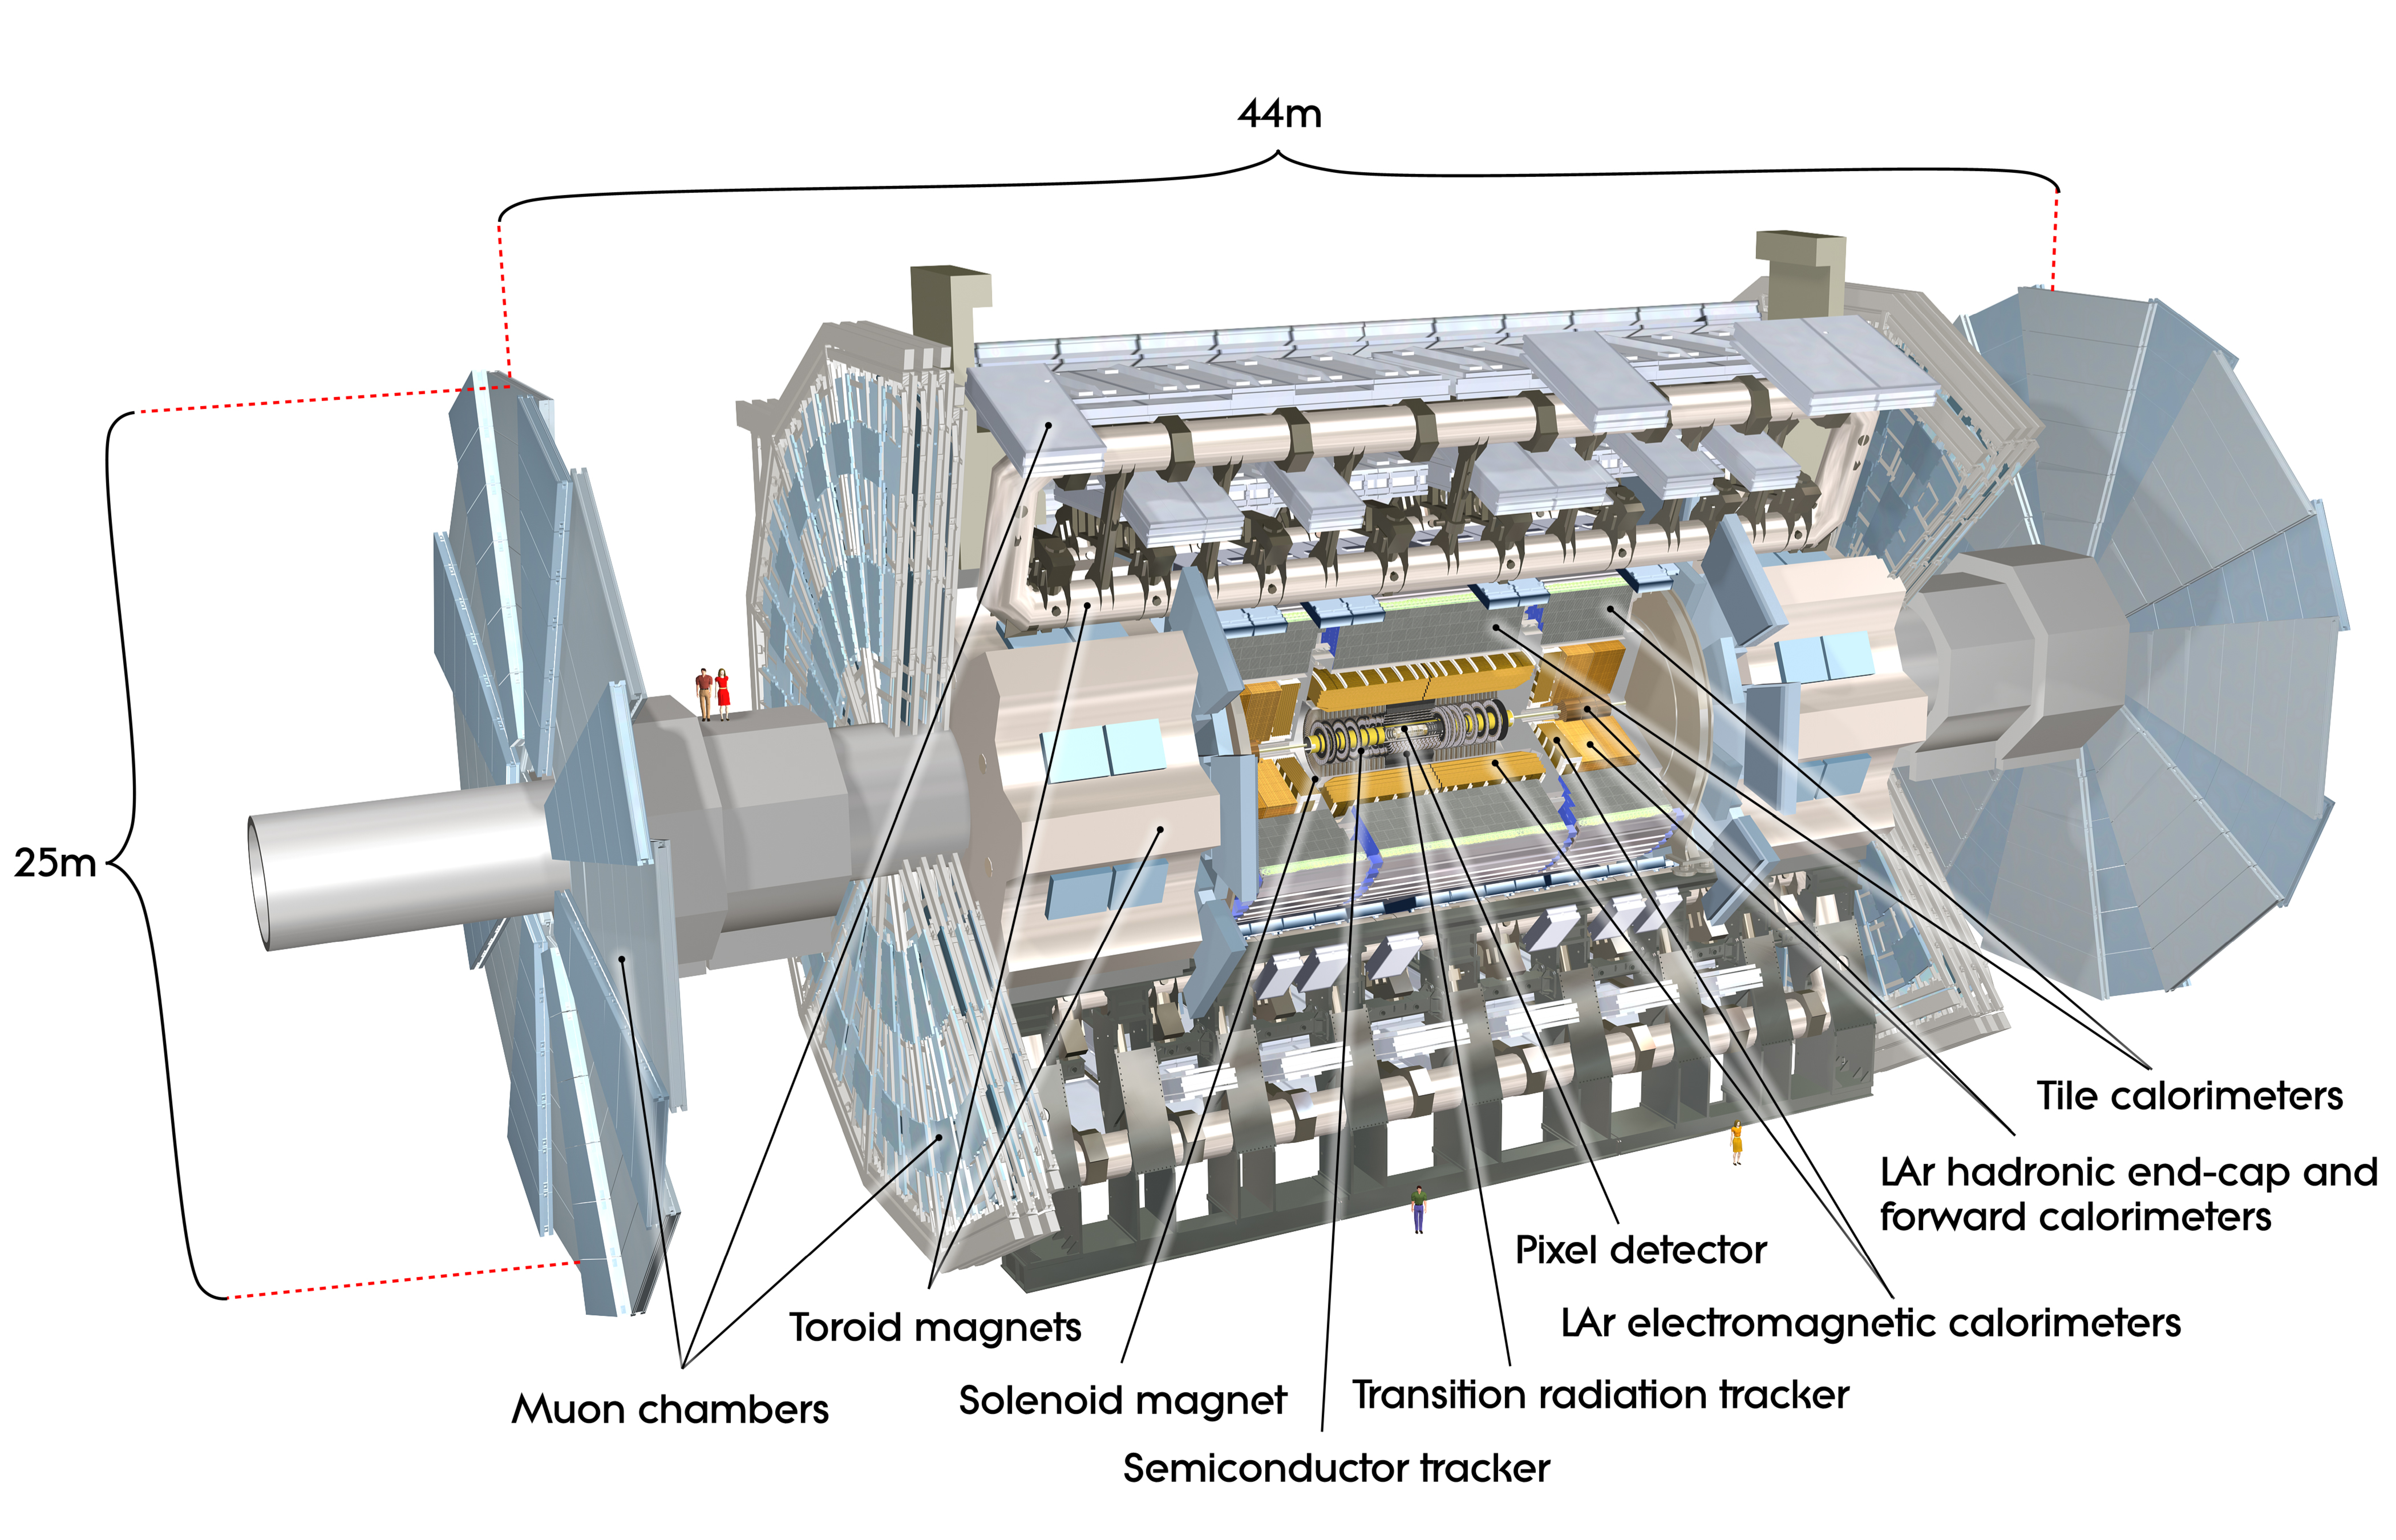
\includegraphics[width=1.0\textwidth]{fig/detector/full_atlas.pdf}
    \caption[]{}
\label{chap:detector:fig:full_atlas}
\end{figure}

The resulting design of the ATLAS detector is displayed in
figure~\ref{chap:detector:fig:full_atlas}. Lying closest to the
collision point, the inner detector (ID) is the primary tracking
system. To resolve the momentum of charged particles, it is immersed
in a uniform 2 T magnetic field. Beyond the ID are the EM and hadronic
calorimeters which measure the energy photons, electrons, and hadrons
produced in the collision. The outermost detectors comprise the muon
spectrometer (MS) system. These detectors are embedded in a high-bend
toroidal magnetic field, resulting in precision tracking across a
large momentum range. The detector is nominally $\pm z$-symmetric and
has eight-fold azimuthal symmetry due to the toroid magnet system. The
various subsystems are segmented in the $z$ direction into a barrel
region with a concentric cylinder geometry, and two end-cap regions
with components that are ``wheels'' or ``disks'' which fit against the
barrel ends, thereby increasing acceptance. 
